\subsection{La numérisation massive des collections visuelles}

Ces dernières années, nous avons été témoin de l'accélération de la numérisation de larges corpus par les institutions patrimoniales. Grâce à leur mise en ligne, ces objets sont devenus accessible pour tous les usagers partout dans le monde. 

\subsubsection{Bibliothèques, archives et musées numériques}

Cette numérisation de masse des collections a permis l'apparition de plateformes en ligne où consulter les différents objets patrimoniaux. Ces sites web se présentent alors comme des bibliothèques, archives et musées numériques. Leur but est de se rapprocher de l'expérience qu'un utilisateur peut avoir lorsqu'il se rend dans l'institution en présentiel. L'avantage de ces projets est qu'il n'est plus nécessaire de se déplacer pour consulter un objet. Avant, les usagers ne pouvaient pas accéder facilement à des documents conservés dans des institutions en dehors de leur ville, voire parfois de leur pays. Cela a permis la diffusion et l'échange du savoir au niveau mondial.  

Nous pouvons citer plusieurs exemples de ce type de projet.

Pour les musées, nous avons le \textit{Musée numérique des musées de Reims} ainsi que les \textit{Collections en ligne des musées de Paris} qui mettent à dispositions des photographies de leur œuvres. En ce qui concerne les archives, au niveau nationale il y a la \textit{Salle de lecture des archives nationales} et au niveau mondial \textit{Internet Archives}. Pour les bibliothèques, en France nous avons \textit{Gallica} créé par la \gls{bnf} mais aussi les \textit{Bibliothèques numériques de l'Institut de France}. 

\begin{figure}[H]
	\centering
	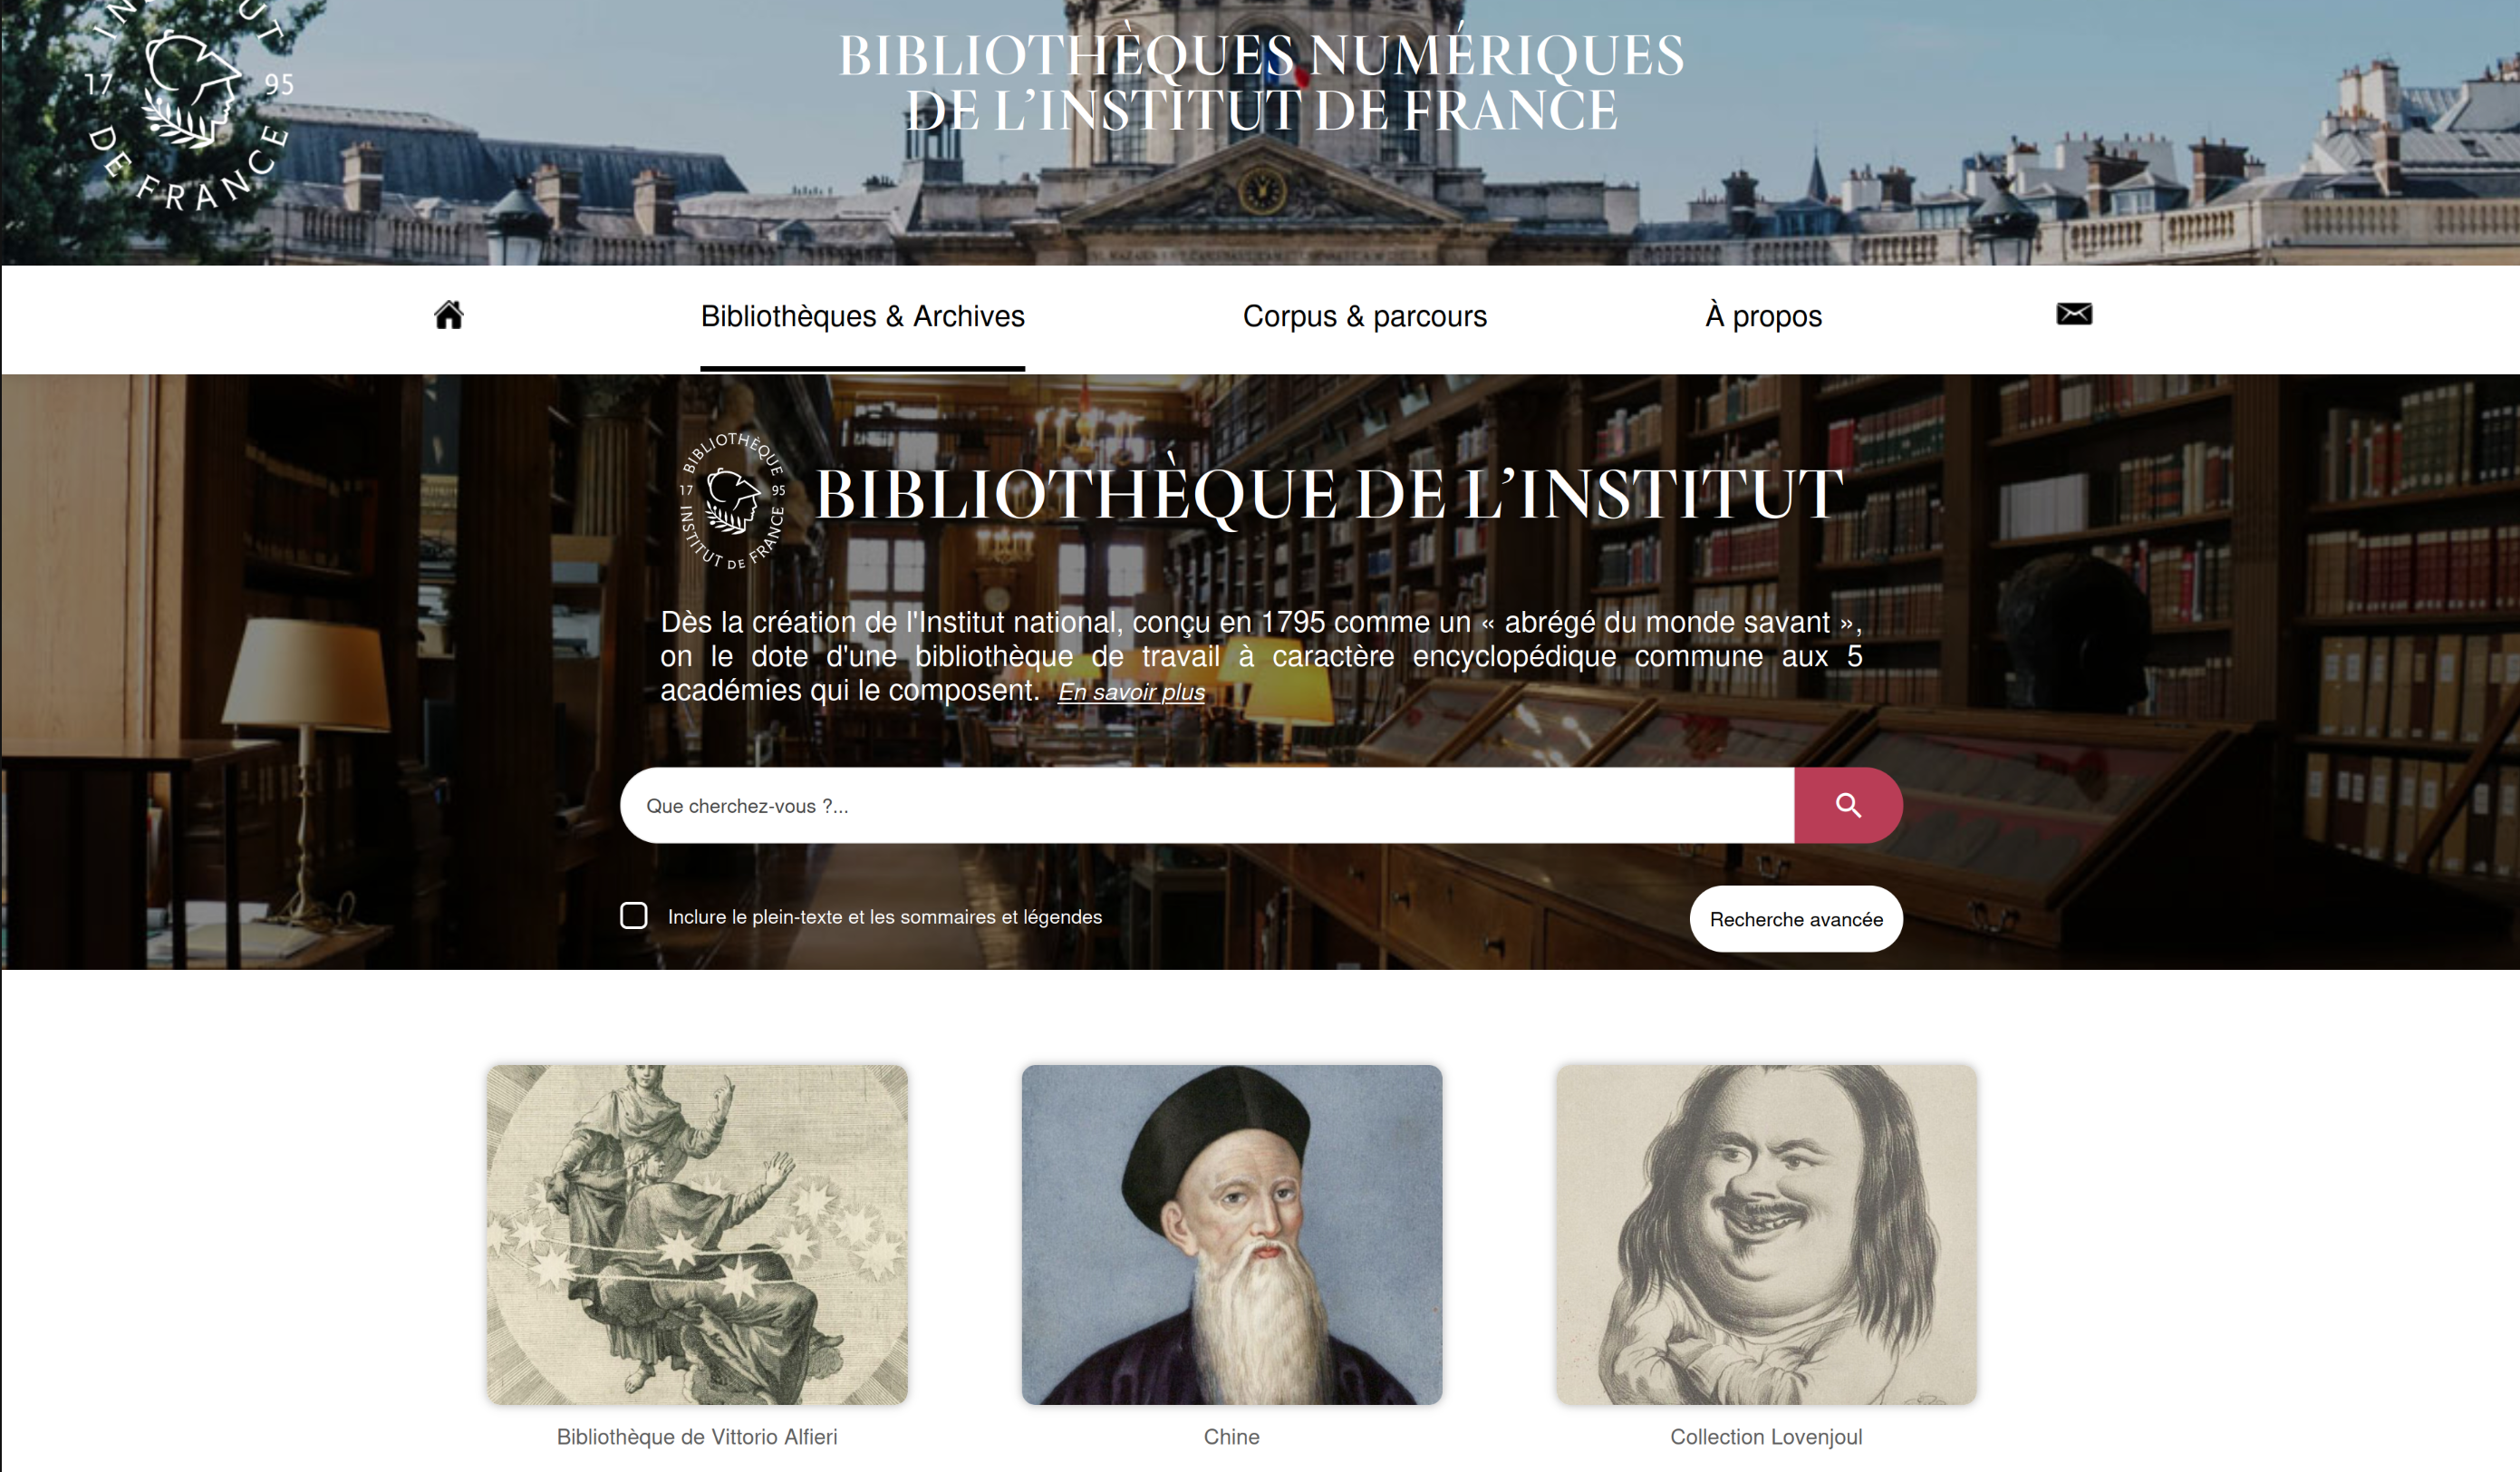
\includegraphics[width=0.8\textwidth]{images/bib_num_institut_france.png}
	\caption{Capture d'écran de la page d'accueil des \textit{bibliothèques numériques de l'Institut de France}}
	\label{fig:institut_france}
\end{figure}

Ces numérisations sont réutilisées par de nombreux projets de recherche comme \gls{eida}.

Cependant, nous y reviendrons plus tard, la création de bibliothèques, archives et musées numériques, nous fait nous questionner sur la manière d'agencer les objets d'un point de vue visuel \footcite{windhagerReviewInformationVisualization}. Faut-il essayer de recréer la disposition des œuvres dans ce type d'institution ou faut-il créer une nouvelle manière de penser l'agencement des objets ? 

Autre point important à signaler : Toutes les numérisations que nous voyons sur les plateformes des institutions n'ont pas été réalisés par ces dernières. Le standard \gls{iiif} permet mettre en place une interopérabilité et un partage des ressources entre les différents acteurs patrimoniaux. 

\subsubsection{Le standard \gls{iiif}} 

Le terme \gls{iiif} désigne à la fois un standard d'interopérabilité mis en place par différentes institutions patrimoniales mais aussi la communauté qui s'est formée autour de lui. Il a été créé pour pallier un manque de collaboration entre les différents grands acteurs du patrimoine qui auparavant rendaient leurs documents visualisables uniquement sur leurs sites web avec leurs propres visualiseurs et méthodes de diffusion\footcite{IIIFDocumentationBiblissima}.

Il est rapidement devenu un consortium international qui se réunit pour élaborer, publier et faire évoluer les spécifications techniques à partir de cas d'usages réels, documentés et partagés. Par la suite, ces principes sont implémentés dans des logiciels et plateformes de diverses natures comme des serveurs d'images, des visualiseurs, des outils d'annotation, des systèmes de gestion de contenu, afin d'assurer leur interopérabilité\footcite{charpierAtelierInitiationIIIF2024}.

Ce standard a pour but de proposer un cadre technique commun afin de diffusion le contenu de manière standardisée. Les images sont alors consultables, manipulables et annotations sur différents logiciels compatibles. Nous pouvons visualiser, zoomer, modifier la taille, appliquer une rotation ou changer le format d'une image via l'\gls{api} Image. Elle permet de manipuler les pixels d'une image à distance à travers une syntaxe d'\gls{url} standardisée. Nous pouvons dès lors faire des requêtes sur l'image. IL est également possible de faire des requêtes d'information sur l'image au format \gls{json}. L'\gls{api} Presentation sert à spécifier des métadonnées pour la présentation d'un objet virtuel via un \textit{manifeste} qui agit comme une \og \textit{enveloppe virtuelle} \fg pour former une unité de distribution élémentaire. Le fichier sera manipulé par des logiciels pour interagir avec la ressource, la visualiser ou la transmettre à un autre outil\footcite{IIIFDocumentationBiblissima}.

Il ne reste plus qu'à adresser une requête \gls{http} avec l'adresse \gls{url} d'une page web au serveur. \gls{iiif} fournit un espace commun pour la recherche et la navigation. Par exemple, un document numérisé par la \gls{bnf} et publié sur \textit{Gallica} peut aussi être visible sur Europeana de cette manière\footcite{charpierAtelierInitiationIIIF2024}.

\subsubsection{Standardisation des métadonnées}

Pour décrire les différents documents numérisés de nombreuses métadonnées sont ajoutées dans leur présentation. Cependant, chaque institution pourrait être tenté d'appliquer leur propre manière méthode en ce qui concerne la descriptions des sources numériques, ce qui va à l'encontre du principe d'interopérabilité. C'est pour cette raison que Europeana a tenté de créer un modèle standardisé : le Europeana Data Model. La documentation présente en ligne nous donne des informations sur les directives de mappages, les modèles d'objets, la définition des classes et des propriétés ainsi que le schéma \gls{xml} pour la validation automatique des métadonnées\footcite{EuropeanaDataModel}. 

\subsection{L'hétérogénéité des objets visuels}

Les objets visuels concernés par ces standards sont multiples et hétérogènes. Nous pouvons les regrouper dans cinq catégories\footcite{windhagerReviewInformationVisualization} : 

\begin{itemize}
	\item Le texte
	\item L'image
	\item La vidéo que nous retrouvons sur le site de l'Institut National de l'Audiovisuel 
	\item Le son
	\item Les objets 3D
\end{itemize}

\subsection{Les différents types d'utilisateurs}

L'article \textit{Visualization of Cultural Heritage Collection Data : State of the Art and Future Challenges} différencie les utilisateurs en deux groupes : les \textit{casual users} et les \textit{experts}.

\subsubsection{Les \textit{Casual users}}

Les \textit{casual users} sont des utilisateurs non spécialisés qui veulent découvrir les collections pour leur culture personnelle. Ils ne connaissent pas forcément le corpus et peuvent vite se retrouver perdus face à la masse de données. Il est donc indispensable de réaliser des interfaces adaptées à eux pour qu'ils puissent entrer dans les collections par le biais d'une thématique ou d'un sous-ensemble. Une interface dont le contenu est uniquement accessible par une barre de recherche pourrait les pénaliser.

\subsubsection{Les \textit{Experts}}

Les \textit{experts} sont des personnes qui connaissent déjà bien le corpus. Ils savent déjà ce qu'ils veulent rechercher. Intégrer une barre de recherche à l'interface est donc une nécessité.

Cependant, contrairement à ce que nous pourrions croire, l'accès aux collections uniquement de cette manière pourrait avoir un impact négatif sur leur recherche. 

Ces dernières années, avec l'arrivée d'Internet, les pratiques de recherche ont été bouleversées. Auparavant, le chercheur partait par le niveau hiérarchique le plus haut comme par exemple un fond d'archives ou une collection de bibliothèque pour ensuite arriver à l'objet recherché. De nos jours, avec l'arrivée de la barre de recherche comme moyen d'accéder aux objets patrimoniaux, la méthode s'est inversée. A présent, le chercheur tape directement le nom ou un mot-clés et il accède au résultat qu'il souhaite. Cependant, en suivant cette méthode, il peut passer à côté d'une découverte importante\footcite{griveauVisualisationDonneesAu2025}. 

Max Kemman affirme que l'influence de Google est l'une des causes de ce problèmes. En effet, ce moteur de recherche nous incite à croire que le seul moyen d'accéder à l'information est la barre de recherche et les mots-clés. Les paramètres avancées sont trop peu souvent utilisées. Il exhorte alors les chercheurs à ne pas se limiter à cette méthode\footcite{kemmanJustGoogleIt2014}.
